\part{Discussion} \label{part:discussion}
\chapter{Discussion} 

\begin{itemize}
	\item Other solutions
	\item Security
	\item What's next
\end{itemize}



\newpage

\chapter{Nfsen, A Graphical Web Tool}

\begin{figure}[!h]
	\centering
	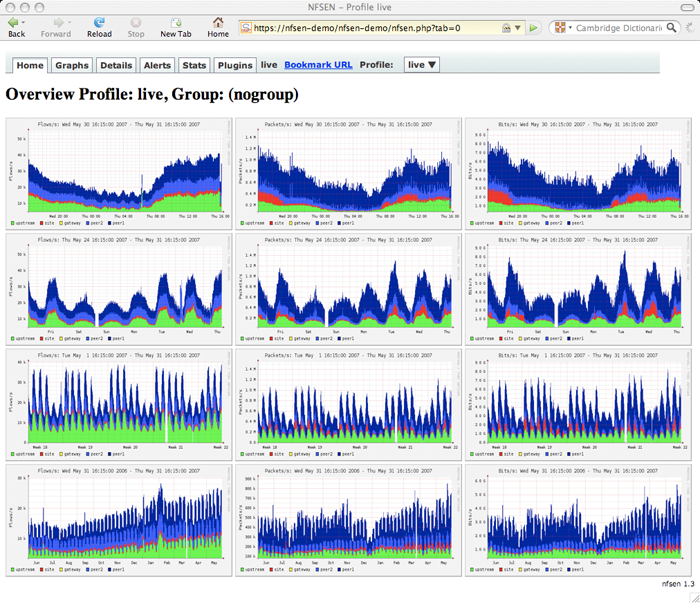
\includegraphics[width=0.8\textwidth]{res/nfsen.png}
	\caption{The Nfsen interface (source : \url{nfsen.sourceforge.net})}
	\label{fig:nfsen}
\end{figure}

The subject of our master thesis having been proposed by Professor Sadre last year and being about monitoring flows in IoT networks, the first tool that was presenting itself to us was Nfsen. Per its official website, \textit{Nfsen is a graphical web based front end for the nfdump netflow tools}. The Nfsen tool uses various graphes and charts to display the traffic of data varying with a specified time span or time interval. It works with the processing capabilities of Nfdump, a data processing tool using Netflow flows that have been retrieved from a network. Specifically, the Nfsen interface also allows to create plugins to have more ways of displaying data information. At first, it was proposed in the description of the subject of the thesis to use Nfsen along with Nfdump, particularly creating an Nfsen addon to show further information along with what Nfsen already is displaying in terms of graphical content. By plugin, one graphical content that Nfsen is lacking is the current topology of the monitored network, which can be added by making a plugin which extends the graphical tool.\\

In this section, we will explain all the underlying layers of Nfsen, from data exchanged in the monitored network to the graphical web page. We will also discuss our thought process about using Nfsen and the reasons why we have not used it in the end.\\

The first step towards monitoring is data collecting. As we explained in Chapter 3, Netflow is used for collecting flows we are interested in, according to some specific attributes such as the source and destination addresses. Once the flow are captured, they are stored and waiting to be processed. \\

(source : http://nfdump.sourceforge.net/, https://www.first.org/conference/2006/papers/haag-peter-papers.pdf)
In reality, when the structure of the Netflow data is defined, the flows are actually captured by \textit{nfcapd}, a \textit{netflow capture deamon}. With nfcapd, the flows are read from the network and the collected data is stored into files, data being split in files according to time slices. Each five minutes, nfcapd outputs a new file where data is stored, named with the current timestamp. One nfcapd process is used for each existing netflow stream that we want to capture.\\

As seen in the next figure, the next important component is \textit{nfdump}. Nfdump is a command line based tool that provides further data processing. Basically, it reads the data that was previously captured and stored by nfcapd. With Nfdump, data is aggregated and it provides further statistics about the traffic. Nfdump can either analyze the data coming from a single file, or from several of them by concatenating them before analyzing. One strength of nfdump is that it can filter out the attributes in the data that are not needed during the processing. Afterwards, the data is output either as a text file or binary data, thus being ready for further analysis. Nfdump aggregates and then creates statistics about the flows information stored, such as traffic volume sent during a timelapse. Nfdump thus acts as the backend of Nfsen.\\

\begin{figure}[!h]
	\centering
	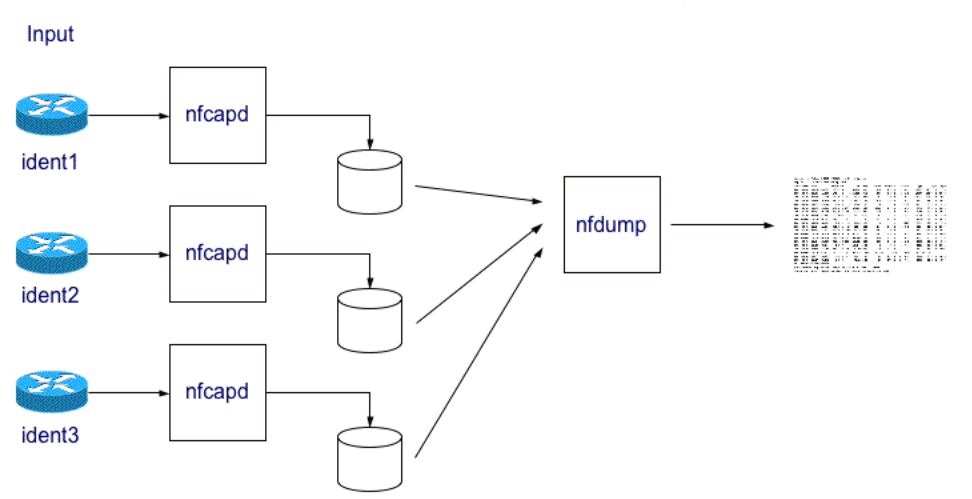
\includegraphics[width=0.8\textwidth]{res/nfdump.png}
	\caption{The Nfdump Structure (source : \url{nfdump.sourceforge.net})}
	\label{fig:nfdump}
\end{figure}

Once the data is processed, it is displayed by Nfsen with the help of graphs. Nfsen displays the collected netflow data, either in flows, packets, or bytes. As you can see in figure \ref{fig:nfsen}, it can display various types of data, for example data sent through different protocols such as UDP, TCP, etc. It also uses time spans to select which data traffic is to be displayed (being the same time spans where nfdump did all the processing).\\

As stated earlier, Nfsen can also be extended, by creating plugins. There exist two kinds of plugins. There are the backend plugins that are written in Perl, that are created to add more functions and functionalities such as alerting conditions and data processing. On the other hand, frontend plugins are written in PHP and used to create new display fashions that the original Nfsen application would lack. In our case, we wanted to display the topology of the network under analysis, which Nfsen is not showing in its original state. Note that each backend plugin should be associated with its respective frontend plugin.

\section{Nfsen \& Nfdump, not best suited?}

In section 5.1, we talked about Nfsen and how it is possible to create plugins to have further monitoring capabilities. As stated, the first description of the thesis was to create an \textit{Nfsen plugin} to visualize an IoT network in an Ad Hoc manner, with devices having Netflow activated.\\

At the beginning of this school year, once we started working on our thesis, we dug into Nfsen and its functionalities, trying to get familiar with it. First of all, setting up the Nfsen tool showed itself to be very tedious and challenging, as many installation tutorials did not work for all computers and OSs, and had different instructions.\\

The main reason why Nfsen is useful is that it easily and immediately treats the netflow information retrieved by nfcapd and nfdump, with little to no addition and/or modification needed. However, as we had decided to modify the netflow structure to visualize IoT networks according to our needs, we also had to modify nfdump. Namely, two fields that the original netflow structure does not monitor, and hence are not standardized fields, are the battery level of devices and the parent of each mote in the IoT networks. Digging into nfdump seems to require quite some time and some knowledge of the Perl language. Entering the last year of our master thesis, we also had never used nor learned the PHP and perl languages in contrary to Javascript with the Node.js framework. \\

Thinking of using the Node.js framework seemed reasonably more practical in our case in terms of time allocation, since we required to modify the netflow information retrieved from networks. With further discussion, we decided to write a Javascript program that played the role of Nfdump to efficiently parse and store the netflow information captured. Similarly, instead of using nfsen as the graphical interface, we programmed a web tool with Node.js to be able to visualize information in which we are interested in. Of course, our graphical interface is less complete than nfsen's, but it contains a topology showcase that nfsen does not, that we have programmed using the D3.js framework as explained earlier.\\

In the end, Nfsen used with Nfdump present a lot of advantages, as most of the work is already present in its core, only a few things have to be added, i.e. the topology here. It contains a lot of graphical information on how much traffic passes through the network, with many filters such as graphs split according to which protocols send the information. But for the reasons we have cited above, we have decided not to use it and opted for a solution using Node.js.

\chapter{Other Possible Solutions}

After having explained the architecture of our monitoring tool and the technologies we have used to implement it, we have also introduced Nfsen along with Nfdump, that was supposed to be the first technology that we were going to use to develop our solution.\\

In this section, we will discuss other possible technologies that could have been used in the place of those that are part of our solution.

TinyOS, RIOT ? 
\newpage
\chapter{Security}

\newpage
\chapter{Possible Extensions}


Data traffic for a specific node, added on a panel, more specific data information for links in the network (with the help of opacity ?), data information for applications in the IoT Network (for now, no application layer?), security (crypted packet, authentication, ...?) 
